\documentclass[article]{aaltoseries}
\usepackage[utf8]{inputenc}


\begin{document}
 
%=========================================================

\title{Deep learning algorithms on mobile devices}

\author{Dongmin Wu
\\\textnormal{\texttt{dongmin.wu@aalto.fi}}} % Your Aalto e-mail address

\affiliation{\textbf{Tutor}: Jukka K. Nurminen} % First and last name of your tutor

\maketitle

%==========================================================

\begin{abstract}

  Since the Deep learning(DL) technology was published, this technology has been
  implemented in various fields and obtained excited results. The Deep learning technology can acquire 
  dependable abstractions from various data, which has benefited different applications, 
  including movement detection, natural language processing and image recognition. 
  Although some of the Deep learning technologies 
  has already reduced the complexity of neural networks to an acceptable size for web service, the 
 scale of the Deep learning technology is still large. 
 According to the high dependency on computation resources,
 Mobile computing devices, such as mobile phone,
  wearable devices and tablet can rarely directly execute the Deep learning technology. 
 Currently, there are already some solutions for implementing DL on mobile\cite{Ota:2017}
 but most of them are focusing on the predicting phase of DL. 
 Discussing the learning phase of DL on mobile is necessary too, 
 it gives a neural network capability of self-evolution without strong help from backend services.

 This paper lists two major solutions currently used in implementing training phase of DL on mobile service;
 briefly introduces the features of both and talks about the scenario of appliance. 


  ----

 a Neural Network will be pre-trained for a special field such as image recognition. 
 The pre-trained N
\vspace{3mm}
\noindent KEYWORDS: Deep learning, mobile devices, training, Dark knowledge

\end{abstract}


%============================================================


\section{Introduction}


Deep learning has been widely used recently. As the main algorithm of Deep learning technology,
 the popularity of neural network algorithm 
 have considerably increased and become the state-of-the art for solving different pattern recognition
problems.

Neural network is inspired by the neural system of the human brain. A neural network will 
try to model pattern of data by using a large number of intelligent nodes, which are named perceptrons. 
After gathering those computational units together, due to the high complexity of neural networks. 
This algorithm has the potential to fetch non-linear features from the training data 
and build a more precise pattern.

As the result, in the image, voice and complex pattern recognition fields, the performance of Deep learning
is generally better then other Machine Learning algorithms.  

However, some obvious issues appeared because of the large complexity of the Deep learning technology. 
Generally, Deep learning algorithms cost most on it training process. 
For example, a typical Convolutional Neural Network (AlexNet \cite{NIPS2012_4824}) 
spends approximately 2.6 minutes in a forward process for one image on a mobile device.  %TODO: reference!
Due to the high computation requirement, Deep learning algorithms mainly run on the Graphics Processing Unit(GPU) or special processors, 

In addition, the energy consumption of Deep learning algorithms is also considerably large. %TODO: [example]

Deep learning also has widely usage scenarios on mobile devices, for example mobile phones, 
wearable devices and vehicle electronics. Mobile devices have less computational resources than 
servers and large computers. On the other hand, mobile devices can hardly afford the energy consumption
of normal Deep learning algorithms. For solving those issues, some approaches appeared.

Ota et al.\cite{Ota:2017}comprehensively listed different Deep learning algorithms,
reviewed some software frameworks and hardware platforms for executing neural networks on mobile devices.
At last they presented some applications running on mobile devices integrated with Deep learning technology. 
But they didn't mention the performance of training a Neural Network on mobile devices. 

%TODO: I should first list some solutions, and then explain that we will compare two of them
This paper will analyses the characteristics of Deep learning and neural network algorithms;
list the different methods of training NN on mobile devices and introduce those methods briefly; 
discuss the pros and cons of each method.
At last, this paper will give a conclusion by supposing some scenarios of appliance.


[structure of paper should combine with last Paragraph]



% 2.1 Problem we faced

% 2.2 how to solve this problem in this paper? --> By comparing different solutions

% 3. Explaination the structure of this paper


%============================================================


\section{Background}

In this section, a brief introduction of Deep learning and mobile devices will be made. Those fundamental 
knowledge helps us to understand the context of this paper better.


%------------------------------------------------------------


\subsection{Deep Learning and neural network}

The neural network in Deep learning can be called Deep Neural Network(DNN), which is one of the most promising 
part of current machine learning methods. 

\subsubsection{History of Deep Neural Network}

% 1. history  1page
Back to middle 1900's there is already a paper introduced a Artificial Neural Network (ANN)\cite{Warren1943}, authors
of that paper raise up the first shallow ANN which mimics the neural network system of human brain. That ANN are not
able to learn models from data, but following researches extended the capabilities of ANN and generated unsupervised 
learning algorithm and supervised algorithm subsequently.

In the 1970s and 1980s, back-propagation learning algorithm was found. Because of efficiency the application of back-propagation
reached its peak in the middle of 80's. LeCun applied this algorithm on the convolutional neural network 
for the first time on 1989, which has significant impact to the Deep learning area. After that, the Cresceptron Model was introduced
and the using of max-pooling layers in the neural network architecture was widely used in modern Deep learning technology.

After the year of 2010, Deep learning has another wave of popularity because there are more affordable GPUs with powerful 
parallel computation capacities. AlexNet\cite{NIPS2012_4824} earned the first prize of 
the 2012 ImageNet Large-Scale Visual Recognition Challenge (ILSVRC). 

From then on, the researching of DNN was considerably accelerated. Google, Facebook, Apple and Amazon has beed published
their own papers in this area. In 2015, Google introduced their GoogLeNet\cite{GoogLeNet}, whose Inception model composing the convolutional 
neural network in a new way that no sequentially arranged layers are possible. In the same year, the ResNet\cite{ResNet} of Microsoft won 
the ILSVRC with the error rate of 3.6\%, which is empirically smaller than the error rate of human beings.




\subsubsection{Characteristic of Deep Neural Network}
% 2. characteristic 1page

The Deep Neural Network higher hierarchy than ANNs, which means a large amount of hidden layers\cite{MAL-006}. 
That difference makes DNN can understand more complex model than ANN, which means the Deep learning or especially DNN
has better behavior on describing non-linear objects, including image, voice, text and bioinformatics.

Besides, comparing to Machine learning technology, deep learning are more suitable for various tasks. The basic concept
of DNN is multi-layers neural network, that algorithm will produce pattern by itself only rely on a large data set
, on the contrary side of some algorithms specifically designed for tasks. With DNN technology, users can tackle different
issue with one implementation of DNN. 

As the widely using of Big data technology, the old machine learning technologies like Support Vector Machine (SVM) are
not such suitable for processing a large amount of data. On the other hand, because of the discovering of back-propagation
algorithm, the efficiency of DNN is relatively higher than traditional Machine learning algorithms.

DNN is more flexible as well. Since the DNN is consisted by multiple neutrons, the amount of neutrons can be adjusted
according to the requirement of different task. This characteristic made DNN has large potential of applying. So far, 
DNN have already impacted our life, services like Google translate, AlphaGo and Siri are the examples of successful applications.






%------------------------------------------------------------


\subsection{Current mobile devices} %2 pages

In this paper, the mobile devices are considered as a group of electronic devices with
computational units that has good mobility and provides the interactive features to human beings.
As the range of mobile is quite large, in this paper, we specifically discuss 3 representative 
mobile devices: Mobile phone, wearable devices and vehicle devices.




%history fo mobile devices
\subsubsection{History of mobile devices}

As the most common mobile devices in our daily life, mobile phone is one of the most familiar 
electronics to normal people. For example, there are nearly 300,000 mobile phones have been 
sold during the second quarter of 2016 \cite{moblePhoneSale}. In 1973 the first handheld mobile phone
was showed by John F. Mitchiell and Martin Copper in America. Since then the mobile phone 
changed the modern life. In 2007, Apple Inc. published the first multi-touch smartphone,
 which made the mobile mobile computation become true.
  Currently, almost all the mobile phones are in this form. 


Wearable devices, like Nike+, Google Glass and Apple watch are produced in the last decade. They presents
a type of on-body electronics in addition to mobile phones. They mainly have specific features, some of them
are designed for monitoring body status while others have limited interactive function.

The last category of mobile devices discussing in this paper is the vehicle devices. From the oldest vacuum tube
car radios to recent automatic driving systems, electronics in vehicles acted an important role while people
driving. Along with the development of mobile electronic technologies, the vehicle devices are becoming more convenient
and computational.



\subsubsection{Characteristic of mobile devices}

Because of the limited resources and specific usage, mobile devices in general do not have a high performance 
universal computation core. Alternatively, they have some specifically designed computation units like DSP processor,
baseband processor and coprocessors.

In mobile phones the power of processors considerably increased in past few years. But the limitation still existed, 
one of the main reason is the energy consumption. Mobile phones has limited size and need meet the requirement continually
using, that limitation makes the computation capability of mobile phones is relatively lower than desktop computers.

As for other wearable devices, they have more limited battery capacity and slower speed. In addition to that, 
they generally have more real-time requirement than mobile phones. Most of them are required to be able to monitoring
movement immediately.

Vehicle devices have the most computation resources comparing to the other two. There are currently some self-driving
car like Waymo exists, most of them are driven by Deep learning technology. But safety requirement of vehicle devices
is highest among others too.  



%------------------------------------------------------------





\section{Challenges of training Neural Network on mobile devices}

This section provides examples of more complex things.


%------------------------------------------------------------


\subsection{computational requirement}
Pruning
Model compression

\subsection{Energy cost}

\subsection{Balance of accuracy and resources consumption}





%------------------------------------------------------------


\section{Current approaches}


% TODO: explain that there already some approaches, but this two of them are most representative. 


To the best of our knowledge, current solutions of squeezing the learning phase of Deep Learning are focusing on two directions:
Reducing the size of Neural Network and Increasing the capability of mobile devices.

There are some representative methods in both directions. 
In this section, two methods will be discussed:
Reducing the size with a mentee Neural Network and Increasing the capability through distributed computation.


\subsection{Reducing the size with a mentee Neural Network}

In 2014, \emph{Knowledge Distillation}, an approach of reducing the size of Neural Network, 
showed an idea of teaching a new simpler Neural Network with a well-trained complex Neural Network.
Within that way, a representative Neural Network was formed and the size is small enough for mobile training.

Figure \ref{fig:mentor_pic}\cite{Distillation:2015} shows the schematic of this mentee-mentor architecture. 

\begin{figure}[t!]
  \begin{center}
    % Note how the file extension has been removed from the filename below
    % so that the LaTeX command can automatically pick any supported file format
    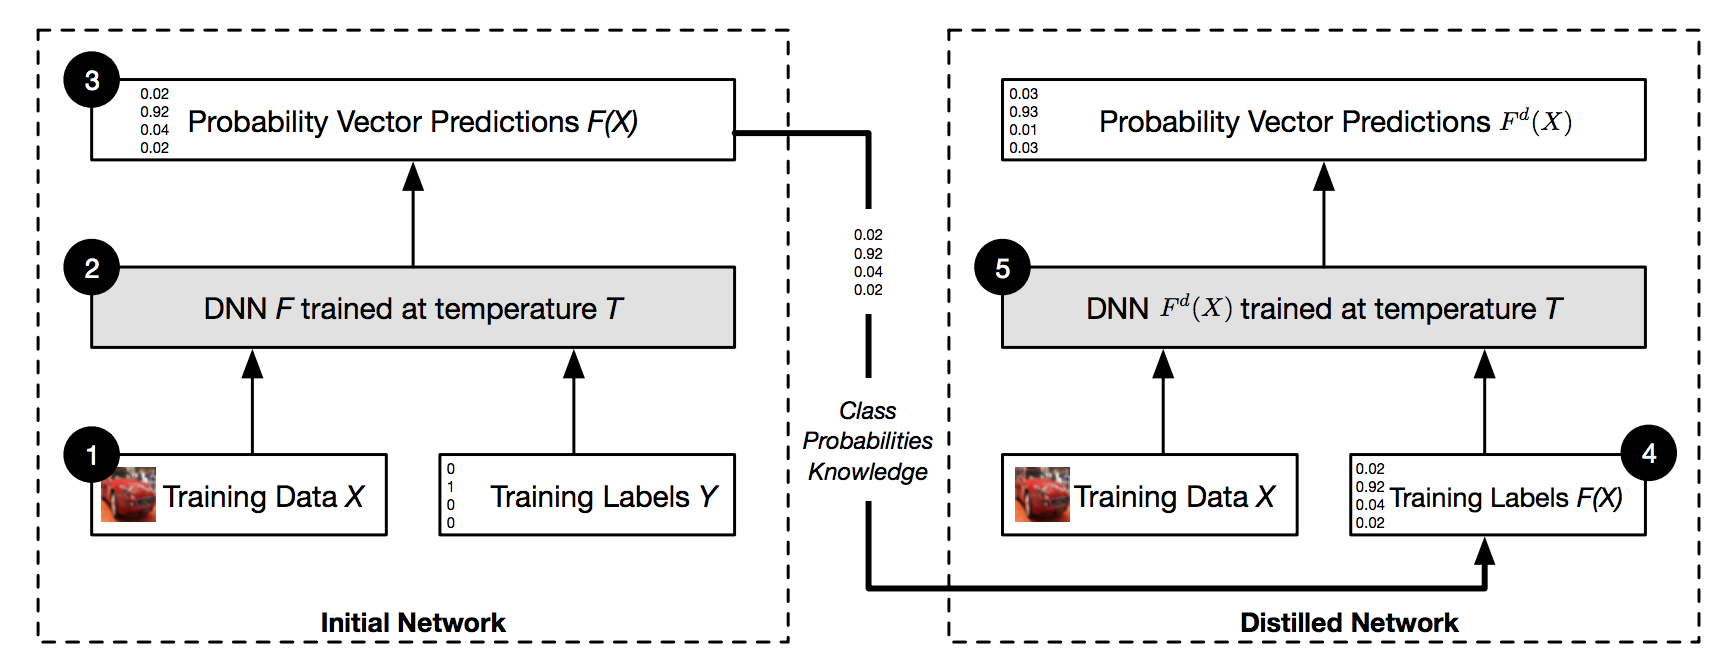
\includegraphics[width=1\textwidth]{figures/mentor_mentee}
    \caption{The mentee network uses the outputs of mentor network as its input labels}
    \label{fig:mentor_pic}
  \end{center}
\end{figure}

As the figure shown, the mentee network has much less layers of Neural Network. 
Hinton et al.[reference], presented the Knowledge Distillation that make neural network smaller by learning the 
output of the softmax layer\cite{SoftMax}. 

This idea was originally introduced by \cite{Caruana2006}, the paper showed 
the output of the softmax layer have much more information than a simply classifier. 
The softmax function are also be able to show the correlations between
target labels. For example, in a computer image recognition neural network for classifying cat, dog and boat.
If the input of that network is a picture of cat, the correlation of the output
between cat and dog is higher than cat versus boat, because the appearance of cat is more similar to dog than boat.
Hinton called those hidden information in the softmax output as \emph{Dark Knowledge}, 
as the knowledge is unused and ignored by normal neural network classifier.

Base on the phenomenon above, a smaller mentee neural network can get more accurate result with the regularization from
the Dark knowledge. 
The approach of \emph{Knowledge Distillation} mainly have two steps: target soften and distillation.

\subsubsection{Target soften}

Normally, for a data set \(X\), we can derive features \(\textbf x \) and correspond target labels \(\textbf y\).
In addition, we can get the predicted output vector \(\textbf y_{mentor}\) from the mentor network.
The parameters in the mentor network is \(\Theta_{mentor}\), 
the derivation of \(\textbf y_{mentor}\) can be represented as below:

%TODO: not sure the equation is correct
%TODO: add softmax function
\[
  \textbf y_{mentor} = softmax(\Theta_{mentor} \textbf{x})
\]

In the practical, the target labels are collected in a format named one-hot, a term comes form the digital
design field\cite{DigitalDesign}. For example, if \(X\) has three target labels: \emph{cat, dog} and \emph{car},
The target labels \(\textbf{y}\) will be presented in following format:

\[
  cat:\ y = \{1,0,0\};\ 
  dog:\ y = \{0,1,0\};\ 
  car:\ y = \{0,0,1\};\ 
\]

The one-hot form above was defined as \emph{hard target}, as they only reveal the classification result of input data.

However, a prediction of a well-trained mentor network \(\textbf y_{mentor}\) will shown as a value between 
\(0\) and \(1\), because of the softmax layer of the neural network. 

\begin{equation} \label{eq:cat_example}
  cat:\ y_{mentor} = \{0.9,0.2,2 \times 10^{-6}\}
\end{equation}

Above is an example output with an input of cat image, 
the first item is obviously highest and the second item is relatively higher than the third.


In the target soften step, 
the output from complex mentor network \(\textbf y_{mentor}\) will be soften in order to get the correlation between categories
by replace the softmax function as below.

\begin{equation} \label{eq:new_soft_max}
  f(z_{(i)}) = \frac{exp(z^{(i)}/T)}{\sum_{j=0}^{N}exp(z^{(j)}/T)}\ for\ i=0,1,...,N
\end{equation}

There, \(T\) represents the "\emph{temperature}" of the soften procedure, a larger \(T\) leads to a more average result. 
If \(T =1\), the equation \ref{eq:cat_example} is the same with normal softmax function. 


\subsubsection{Distillation}

The aim of distillation is to transfer the knowledge from the larger mentor neural network to the mentee. 
The mentee will use the output of the mentor with high temperature as the target labels.
Equally, the softmax layer of the mentee neural network has the same temperature with its mentor.

As the result, the cross-entropy between the mentee and mentor presents as:

\begin{equation} \label{eq:cost_function}
  C(y_{mentee}, y_{mentor}) = - \sum y_{mentor}log(y_{mentee})
\end{equation}

Insert equation \ref{eq:new_soft_max} into equation \ref{eq:cost_function}, we can derivate below:

\begin{equation} \label{eq:cost_function1}
  C(y_{mentee}, y_{mentor}) = - \sum_i f(v_i)log(f(z_i))
\end{equation}

There, \(v_i,\ z_i\) presents the input of mentor and mentee's softmax layer respectively.

Thus, the gradient of equation \ref{eq:cost_function1} is:

\begin{equation} \label{eq:gradient_cost}
  \frac{\nabla C}{\nabla z_i} = \frac{1}{T}(f(v_i) - f(z_i))
\end{equation}

Expand equation \ref{eq:gradient_cost}, while \(T\) is large enough, the equation transform into below:

\begin{equation} \label{eq:gradient_cost1}
  \frac{\nabla C}{\nabla z_i} \approx \frac{1}{T}( \frac{1+z_i/T}{N+\sum_j z_i/T} - \frac{1+v_i/T}{N+\sum_j v_i/T} ) = \frac{1}{T} (\frac{z_i - v_i}{N})
\end{equation}

Within the cost function \ref{eq:cost_function1} and the gradient equation \ref{eq:gradient_cost1}, 
the mentee neural network can learn the knowledge from its mentor.

The Dark Knowledge introduced an good approach for mobile training. 
A large and well-trained Neural Network, which has a general knowledge of a scenario, can be computed and stored in the powerful server cloud.
At the meantime, a small mentee network regularized by the mentor network can be stored and tuned on the mobile devices.
For a specific use case, the mentee network is able to learn from that and adjust the predict result. 



% Maybe I can move this part to another section
The advantage of this method is obvious, 
the size of mentee network is much smaller than the mentor network but has similar performance
with the complex mentor network. 
Although this compression is efficiency, the mentee network can still too large to for some mobile
devices such as wearable devices.

%TODO: add disadvantage of dark knowledge/knowledge Distillation
%TODO disadvantage of knowledge distillation
%   1. the performance is bad on small set of categories
%   2. not efficient on GAN neural network

\subsection{Federal learning among multiple mobile devices}


%------------------------------------------------------------




%============================================================


\section{Conclusion}

To be added.


%============================================================


\bibliographystyle{plain}
\bibliography{cs-seminar}

\end{document}
